\begin{tikzpicture}[domain=0:2.5]
	% Achsen zeichnen
	\draw[->,thick] (0,0) -- (5,0) node[right] {$ k$};
	\draw[->,thick] (0,0) -- (0,3) node[above] {$\omega( k)$};
	%Plot
	\draw plot (\x,{0.2*exp(\x)-0.2});
	% Beschriftung
	\draw (-.1,1.25) -- (.1,1.25) node[left=4pt] {$\omega_0$};
	\draw (2,-.1) -- (2,.1) node[below=4pt] {$ k_0$};
	\draw[style=dashed] (.2,1.25)--(2,1.25) node[right=8pt] {$ v_{\mathrm{g}}$} -- (2, .2);
	\draw (1.25,0.25)--(2.75,2.25);
\end{tikzpicture}
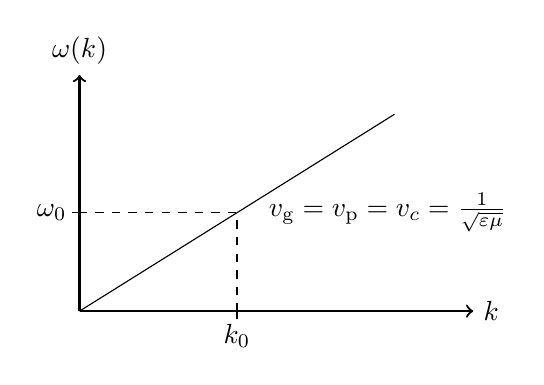
\begin{tikzpicture}
	% Achsen zeichnen
	\draw[->,thick] (0,0) -- (5,0) node[right] {$ k$};
	\draw[->,thick] (0,0) -- (0,3) node[above] {$\omega( k)$};
	% Plott
	\draw (0,0) -- (4,2.5);
	% Beschriftung
	\draw (-.1,1.25) -- (.1,1.25) node[left=4pt] {$\omega_0$};
	\draw (2,-.1) -- (2,.1) node[below=4pt] {$ k_0$};
	\draw[style=dashed] (.2,1.25)--(2,1.25)node[right=8pt] {$ v_{\mathrm{g}}= v_{\mathrm{p}}= v_{c} = \frac{1}{\sqrt{\varepsilon\mu}}$} -- (2, .2);
\end{tikzpicture}